% Elsevier elsarticle manuscript skeleton; content is added only after author approval.
% Source template: Desktop/论文修改/写作/elsarticle/elsarticle-template-num.tex
\documentclass[final,5p,times,twocolumn]{elsarticle}

\usepackage{amsmath,amssymb}
\usepackage{graphicx}
\usepackage{booktabs}
\usepackage{multirow}
\usepackage{algorithm}
\usepackage{algpseudocode}
\usepackage{float}
\usepackage{placeins}
\usepackage{dblfloatfix}
\usepackage{hyperref}
\hypersetup{hidelinks}
\usepackage{CJKutf8}
\providecommand{\methodrevision}[1]{#1}

% Keep double-column floats close to their discussion and avoid sparse float pages.
\renewcommand{\topfraction}{0.95}
\renewcommand{\bottomfraction}{0.90}
\renewcommand{\textfraction}{0.05}
\renewcommand{\floatpagefraction}{0.80}
\renewcommand{\dbltopfraction}{0.95}
\renewcommand{\dblfloatpagefraction}{0.80}
\setlength{\textfloatsep}{10pt plus 2pt minus 2pt}
\setlength{\dbltextfloatsep}{10pt plus 2pt minus 2pt}
\setcounter{topnumber}{3}
\setcounter{bottomnumber}{2}
\setcounter{totalnumber}{5}
\setcounter{dbltopnumber}{2}
\makeatletter
\setlength{\@fptop}{0pt}
\setlength{\@fpsep}{12pt}
\setlength{\@fpbot}{0pt plus 1fil}
\makeatother

\journal{Knowledge-Based Systems}

\begin{document}
\begin{frontmatter}

\title{Sample-Adaptive Relational Knowledge Integration for Zero-Shot Audio Classification}

\author[inst1]{Kexin Zhang\fnref{equalcontrib}}
\ead{25461355022@stu.wzu.edu.cn}

\author[inst2]{Zhizhong Ma\fnref{equalcontrib}}
\ead{mazhizhong@wzut.edu.cn}

\author[inst2]{Yitian Lin}
\ead{yitian.lin@wzut.edu.cn}

\author[inst2]{Bingchen Lin\fnref{orcidlin}}
\ead{Bingchen.Lin@wzut.edu.cn}

\author[inst3]{Haihan Yang}
\ead{269964500@stu.cwnu.edu.cn}

\author[inst2]{Zhengqiu Weng\corref{corresponding}}
\ead{derisweng@wzut.edu.cn}

\author[inst1,inst4]{Hui Huang\corref{corresponding}}
\ead{huanghui@wzu.edu.cn}

\fntext[equalcontrib]{Kexin Zhang and Zhizhong Ma contributed equally to this work.}
\fntext[orcidlin]{ORCID: \href{https://orcid.org/0000-0002-7046-7189}{0000-0002-7046-7189}.}
\cortext[corresponding]{Corresponding authors: Zhengqiu Weng and Hui Huang.}

\affiliation[inst1]{organization={College of Computer Science and Artificial Intelligence, Wenzhou University},
  city={Wenzhou}, postcode={325035}, country={China}}
\affiliation[inst2]{organization={School of Data Science and Artificial Intelligence, Wenzhou University of Technology},
  city={Wenzhou}, postcode={325035}, country={China}}
\affiliation[inst3]{organization={School of Electronic Information Engineering, China West Normal University},
  city={Nanchong}, postcode={637009}, country={China}}
\affiliation[inst4]{organization={Wenzhou Turing Institute for Advanced Study in Artificial Intelligence},
  city={Wenzhou}, postcode={325035}, country={China}}

\begin{abstract}
\begin{CJK*}{UTF8}{gbsn}
零样本音频分类通过匹配音频与自然语言类别描述，使预训练模型无需针对目标任务重新训练即可识别声音。然而，简短的类别名称难以充分表达声音事件的来源、场景及语义联系，限制了音频--文本匹配所能利用的信息。知识图谱能够补充这些语义联系，但如何选择适合当前音频的知识、准确表达关系语义并协调其对分类决策的影响，仍是知识增强中的关键问题。为此，本文提出样本自适应知识整合框架（Sample-Adaptive Knowledge Integration，SAKI），在保持对比语言--音频预训练模型（CLAP）参数不变的条件下，利用结构化知识改善候选类别排序。该框架通过音频对齐知识语言化模块（Audio-Aligned Knowledge Verbalization，AAKV），利用声音导向指令和实体--关系约束，引导大语言模型将三元组转换为自然语言证据；在此基础上，将不同关系下的知识增强预测构建为关系专家，结合预测共识与分类间隔，无需测试标签即可选择适合当前音频的关系；随后，在类别内部聚合所选知识证据，并与原始CLAP分数进行分层融合。\methodrevision{在五个公开音频数据集上，SAKI相较于本文复现的iKnow-audio，Hit@1提高了2.08--12.73个百分点，MRR提高了1.02--6.68个百分点。}本文将类别关联的结构化知识转化为面向当前音频的判别证据，为缓解类别描述的语义不足、实现样本自适应的知识增强提供了统一框架。
\end{CJK*}
\end{abstract}

\begin{keyword}
Zero-shot audio classification \sep CLAP \sep Audio-centric knowledge graph \sep Sample-level relation selection \sep Knowledge verbalization \sep Evidence fusion
\end{keyword}

\end{frontmatter}

\section{Introduction}\label{sec:introduction}
\begin{CJK*}{UTF8}{gbsn}

\nextrevision{零样本音频分类旨在利用类别语义识别缺少目标任务训练样本的声音类别，从而减少对音频标注数据的依赖。早期方法通过匹配音频表示与类别语义嵌入，实现对未见类别的识别~\cite{xie2021zero}。对比语言--音频预训练模型（Contrastive Language--Audio Pretraining，CLAP）进一步通过大规模音频--文本对比学习建立共享表示空间，使自然语言描述能够直接用于声音分类~\cite{elizalde2023clap}。后续研究通过扩充训练数据、改进预训练目标及音频建模方式，持续增强音频--语言表示与零样本泛化能力~\cite{wu2023clap,niizumi2024m2dclap,mei2026slap}。然而，当类别主要由简短名称表示时，声音的来源、发生场景及其与其他事件的语义联系难以得到充分表达，限制了分类过程中可利用的判别信息。}

\nextrevision{为丰富类别的语义表示，已有研究从文本提示和结构化知识两个方向展开探索。ReCLAP通过改写音频描述和生成类别增强提示，补充声音特征与场景信息；PAT根据输入音频选择和组合提示，并调整音频表示，以改善音频与文本的匹配~\cite{ghosh2024reclap,seth2025pat}。这些工作从不同角度说明了文本内容及其与输入音频的适配对零样本分类的重要性。结构化知识则提供了另一种补充语义信息的途径。iKnow-audio构建音频中心知识图谱（Audio-centric Knowledge Graph，AKG），通过经过筛选的关系集合检索与候选类别相关的尾实体，并将其与类别名称组合为增强提示，用于修正CLAP的候选排序~\cite{olvera-etal-2025-iknow}。该研究展示了将声音事件之间的结构化联系引入零样本音频分类的可行性，也进一步引出了如何使图谱知识适配具体音频的问题。}

\nextrevision{尽管上述研究丰富了零样本音频分类可利用的语义信息，图谱知识在具体样本上的选择、表达与融合仍有进一步改进的空间。首先，经过筛选的关系集合能够提供类别相关知识，但同一关系对不同音频样本的判别价值可能不同，仍需根据当前音频确定参与知识增强的关系。其次，iKnow-audio通过拼接类别名称与检索到的尾实体构造增强提示，未显式保留连接二者的关系语义，因而需要一种能够表达实体间关系、同时约束额外内容扩写的文本构造方式。最后，在分数融合方面，原始类别分数与增强提示分数被共同聚合，知识证据的汇总与其对基础预测的影响在同一聚合过程中确定，缺少对这两个环节的分别控制。当某一类别的知识提示数量较多或匹配分数较高时，知识证据可能对聚合结果产生过大影响，使原始CLAP预测的作用难以单独调节。因此，如何依据当前音频选择关系、完整表达所选知识的关系语义，并分别组织知识证据聚合与原始预测融合，是本文关注的问题。}

\nextrevision{针对上述问题，本文提出样本自适应知识整合框架（Sample-Adaptive Knowledge Integration，SAKI），在保持CLAP参数不变的条件下，利用结构化知识改善候选类别排序。在离线阶段，音频对齐知识语言化模块（Audio-Aligned Knowledge Verbalization，AAKV）引导大语言模型在保留实体及关系语义的前提下，将检索得到的三元组改写为以声音为主体的自然语言描述，并缓存对应的文本向量。在在线阶段，SAKI为每种关系构建一个利用该关系知识进行分类的关系专家，依据专家间的预测共识与各专家的分类间隔，选择参与当前音频分类的关系。随后，框架聚合所选关系提供的知识证据，并与原始CLAP分数进行分层融合，完成候选类别重排序。该框架无需利用目标数据集的训练样本训练关系选择器，在线推理过程不使用测试标签。}

本文的主要贡献如下：
\begin{itemize}
  \item \nextrevision{提出样本级关系选择方法，利用关系专家的预测信息，使参与知识增强的关系随输入音频调整。}
  \item \nextrevision{提出AAKV，在保留实体与关系语义的基础上，将图谱三元组转化为面向音频匹配的文本证据。}
  \item \nextrevision{构建分层知识融合机制，协调知识证据与原始CLAP预测，并通过跨数据集对照与消融实验评估完整框架及各模块的作用。}
\end{itemize}

\nextrevision{本文在五个公开音频数据集上开展评估。相较于受控复现的iKnow-audio，SAKI的Hit@1提高了2.08--12.73个百分点，MRR提高了1.02--6.68个百分点。组合消融结果显示，完整配置取得最高的五数据集等权平均Hit@1和MRR；关系选择与知识语言化对照进一步检验了相应模块的作用。此外，本文通过统计分析、逐样本预测变化、参数敏感性及计算成本分析，考察方法的性能收益与适用边界。}

\nextrevision{本文其余部分安排如下：第2节介绍相关研究，第3节阐述SAKI的总体框架及三个核心模块，第4节报告实验设置、主要结果与进一步分析，第5节讨论主要发现与研究局限，第6节总结全文。}

\end{CJK*}

\providecommand{\methodrevision}[1]{#1}
\section{Related work}\label{sec:related-work}
\begin{CJK*}{UTF8}{gbsn}

\subsection{Zero-Shot Audio Classification with Audio--Language Models}

零样本音频分类研究关注如何在目标类别缺少训练音频的情况下，利用类别语义完成声音识别。早期方法通常将音频表示与由 Word2Vec、GloVe 或 BERT 等语言模型获得的类别语义嵌入进行匹配，并通过兼容性函数预测训练阶段未出现的类别~\cite{xie2021zero}。随着视觉--语言预训练的发展，CLIP 通过图像编码器和文本编码器建立共享表示空间，为利用自然语言进行零样本识别提供了通用范式~\cite{radford2021learning}。AudioCLIP 将音频模态引入 CLIP，使音频、图像和文本能够在统一空间中进行匹配；Wav2CLIP 则通过从 CLIP 视觉表示中蒸馏音频表示，使音频嵌入与图像和文本嵌入保持对齐，并支持零样本分类与跨模态检索~\cite{guzhov2021audioclip,wu2022wav2clip}。这些研究逐步将零样本音频分类从类别语义匹配扩展为音频、图像和文本之间的跨模态推理。

CLAP 进一步通过大规模音频--文本对比学习直接建立音频与文本之间的语义对应关系，为零样本音频分类提供了音频--语言推理框架~\cite{elizalde2023clap}。后续模型主要从训练数据、预训练目标和模型结构等方面扩展音频--语言表示能力，例如引入大规模音频--文本数据和文本增强策略，将掩码建模与跨模态对齐结合，或面向可变长度音频进行训练~\cite{wu2023clap,niizumi2024m2dclap,mei2026slap}。在上述音频--语言推理框架中，类别文本不仅用于标识候选类别，其具体语义内容也会参与音频--文本相似度计算，并影响最终的类别排序。与此同时，类别之间的结构关系通常没有被显式纳入这一分类过程。

\subsection{Textual Prompting and Sound Semantic Description}

为丰富类别文本中的声音语义，已有研究从声音属性建模和类别描述扩展两个方面改进文本表示。Binary Attribute Embeddings 将音高、持续时间和材质等声音属性编码为类别语义表示~\cite{lin2022binary}；Sound Attribute Vector 进一步结合全局和局部特征学习声音属性，以增强类别语义与局部声学模式之间的联系~\cite{lin2023soundattribute}。随后，语言模型被用于生成更加完整的声音属性知识，类别文本也开始加入具有区分度的声学特征和场景信息~\cite{xu2024soundattribute,ghosh2024reclap}。这类方法将类别文本从简单标签扩展为包含声音属性和场景信息的描述，以改善文本内容与输入音频之间的语义匹配。

另一类研究从任务信息和输入信息出发构造更加适配的提示。TSPE 将类别标签、声音属性和声源信息组合为任务相关的提示集合~\cite{anand2025tspe}；PAT 根据输入音频选择和组合提示，并对音频特征进行相应调整~\cite{seth2025pat}；AudioCards 则利用结构化元数据、声学属性和声音描述生成面向音频内容的文本卡片~\cite{sridhar2026audiocards}。这些研究推动了音频文本从静态类别标签向属性化、任务相关和内容相关的表达形式发展。其中，ReCLAP、TSPE、PAT 和 AudioCards 主要从描述、提示或结构化元数据的构造方式改善文本输入；如何将外部语义信息转换为与当前音频匹配的文本证据，仍缺少统一的表达方式。

% Queue the method overview early so it appears at the top of page 3.
\providecommand{\methodframeworkfigure}{figures/saki_framework.png}
\providecommand{\methodframeworkwidth}{0.96\textwidth}
\begin{figure*}[!t]
  \centering
  \includegraphics[width=\methodframeworkwidth]{\methodframeworkfigure}
  \caption{\methodrevision{Overview of SAKI. Retrieved graph triples are verbalized and encoded offline. At inference, CLAP first ranks all candidate classes; relation experts then produce a Top-1 prediction and top-two score gap for the current audio. The consensus class and expert gaps determine the selected relations. Their cached evidence is aggregated by class and combined with the original CLAP scores for final ranking.}}
  \label{fig:framework}
\end{figure*}

\subsection{Structured Knowledge and Evidence-Aware Candidate Ranking}

结构化知识为音频理解提供了类别层级、事件属性和场景关系等显式语义信息。AudioSet 通过层次化本体组织大规模音频事件类别，为音频标签之间的语义关联提供了统一结构~\cite{gemmeke2017audioset}。基于本体的神经网络利用类别层级或本体关系约束声音事件分类，ontology-aware 音频事件分类方法进一步将标签依赖关系纳入分类模型~\cite{jimenez2018ontology,sun2020ontology}。在此基础上，图节点嵌入方法将类别关系表示为节点结构，并研究节点表示对音频分类的影响；事件关系图则将声学事件作为图节点，并利用边特征描述场景中的事件关联~\cite{aironi2022graph,hou2023audio}。这些研究表明，类别层级、标签依赖和事件关系能够为音频分类提供补充语义信息；iKnow-audio 进一步将此类结构化知识用于 CLAP 候选预测。

知识图谱嵌入方法进一步为实体--关系组合提供可计算的合理性评分。RotatE 在复数空间中将关系建模为旋转操作，用于知识图谱嵌入和链接预测~\cite{sun2019rotate}。iKnow-audio 将音频中心知识图谱引入 CLAP 推理过程，利用图谱中的相关实体补充候选类别预测~\cite{olvera-etal-2025-iknow}。在预训练模型适配研究中，CLIP-Adapter 通过残差式特征混合将附加分支与原始 CLIP 表示结合，Tip-Adapter 则利用键值缓存中的外部信息修正 CLIP 的原始预测~\cite{gao2021clipadapter,zhang2022tipadapter}。这些研究从图谱表示、实体检索和外部信息融合等方面展示了结构化知识参与候选预测的可行性。

样本相关的知识选择也已在视觉分类中得到研究。Tang 等人提出 SINet，通过基于注意力的知识选择模块根据图像特征筛选知识图谱中的有效知识，并利用知识选择损失约束知识表示与视觉特征的一致性~\cite{tang2023sinet}。与该类监督图像分类方法不同，本文面向零样本音频分类，利用关系条件预测及其共识与分类间隔，在推理阶段动态确定参与知识增强的关系。

尽管上述研究分别从音频--语言对齐、类别文本表达、结构化知识利用以及样本相关知识选择等角度进行了探索，但其作用对象和推理设置并不相同。特别是在零样本音频分类场景中，如何在不利用目标数据训练样本条件选择器的情况下，根据当前音频动态确定知识关系优先级，并进一步协调关系证据的文本表达方式以及知识分数与原始 CLAP 分数的融合，仍缺少统一的处理机制。本文沿着这一研究脉络，将样本级关系选择、Audio-Aligned Knowledge Verbalization 和分层知识证据融合纳入统一的零样本音频分类流程。

\end{CJK*}

% !TeX root = ../main.tex
\providecommand{\methodrevision}[1]{#1}
\section{Method}\label{sec:method}
\begin{CJK*}{UTF8}{gbsn}

本文面向无需目标数据训练的零样本音频分类，在保留CLAP原始跨模态判别能力的基础上，从音频中心知识图谱中为当前样本选择相关关系证据。图~\ref{fig:framework}给出了整体流程。离线阶段为每个“类别--关系”组合检索候选尾实体，Audio-Aligned Knowledge Verbalization（AAKV）将图三元组转换为受约束的声音描述，并缓存相应的CLAP文本表示。在线阶段首先依据CLAP分数确定待增强的候选类别，再将每种候选关系构建为一个关系专家，利用专家间的预测共识与分类间隔执行样本级关系选择。最后，分层融合模块先聚合知识证据，再与原始CLAP分数结合，得到全部候选类别的最终排序。整个推理过程不使用测试标签。


\subsection{Problem formulation}\label{sec:problem-formulation}

给定输入音频$x^a$和由$N$个类别构成的候选集合$\mathcal C=\{c_1,c_2,\ldots,c_N\}$，零样本音频分类的目标是在不利用目标数据集训练样本的条件下，为每个候选类别计算预测分数，并输出排序最高的类别：
\begin{equation}
\hat y=\arg\max_{c_i\in\mathcal C}s_{\mathrm{final}}(c_i\mid x^a),
\label{eq:prediction}
\end{equation}
其中，$\hat y$为最终预测类别，$s_{\mathrm{final}}(c_i\mid x^a)$为类别$c_i$的\methodrevision{最终类别分数}。本文采用预训练的CLAP音频编码器$f_a(\cdot)$和文本编码器$f_t(\cdot)$。结构化知识由音频中心知识图谱$\mathcal G=(\mathcal E,\mathcal R,\mathcal T)$提供，其中$\mathcal E$、$\mathcal R$和$\mathcal T$分别为实体集、关系集和三元组集合。\methodrevision{下表汇总方法部分反复使用的主要记号。}

\par\smallskip\noindent\begin{minipage}{\columnwidth}
\methodrevision{%
\centering
\textbf{主要记号及其含义}\par\smallskip
\footnotesize
\setlength{\tabcolsep}{4pt}
\begin{tabular}{@{}p{0.37\columnwidth}p{0.55\columnwidth}@{}}
\toprule
记号 & 含义 \\
\midrule
$x^a,\mathcal C,c_i$ & 输入音频、候选类别集合及其中的类别 \\
$\mathcal G,\mathcal E,\mathcal R$ & 知识图谱、实体集合及关系集合 \\
$K,M,N_r$ & 初始候选类别数、每个类别--关系的尾实体上限、最终选择的关系数 \\
$s_{\mathrm{base}},s_r,s_{\mathrm{final}}$ & 原始CLAP分数、单关系专家分数、最终类别分数 \\
$\mathcal E_{i,r},\mathcal U_{i,r}$ & 类别--关系的有效尾实体及其证据分数序列 \\
$\mathcal U_i^*$ & 所选关系合并去重后的证据分数序列 \\
$A_{\lambda},\lambda$ & 知识证据聚合算子及其固定尺度 \\
$\mathcal F,\alpha$ & 分层融合规则及原始CLAP分数的权重 \\
\bottomrule
\end{tabular}
}
\end{minipage}\par\smallskip

\subsection{CLAP initial retrieval and graph evidence construction}\label{sec:initial-retrieval}

给定输入音频$x^a$和类别文本$c_i$，将CLAP输出的音频表示和文本表示进行$L_2$归一化，分别记为$\mathbf e^a$和$\mathbf e_i^t$。\methodrevision{沿用CLAP的音频--文本相似度计算~\cite{elizalde2023clap}，}二者的基础跨模态分数为
\begin{equation}
s_{\mathrm{base}}(c_i\mid x^a)=(\mathbf e^a)^\top\mathbf e_i^t.
\label{eq:base-score}
\end{equation}
按照$s_{\mathrm{base}}$对全部候选类别排序，得到接受知识增强的候选集合
\begin{equation}
\mathcal C_K(x^a)=\operatorname{TopK}_{c_i\in\mathcal C}s_{\mathrm{base}}(c_i\mid x^a).
\label{eq:topk}
\end{equation}
其中，$K$为接受知识增强的初始候选类别数。知识增强仅作用于$\mathcal C_K$；其余类别保留基础分数，并共同参与最终排序。

\methodrevision{类别$c_i$根据预先核验的类别--实体映射对应图谱头实体$h_i\in\mathcal E$；未能映射的类别不引入图知识。}遵循iKnow-audio的知识检索设置，本文使用预训练的RotatE知识图谱嵌入模型对候选三元组进行评分~\cite{olvera-etal-2025-iknow,sun2019rotate}。给定头实体$h_i$和关系$r\in\mathcal R$，$\phi_{\mathrm{KG}}(h_i,r,t)$表示候选三元组$(h_i,r,t)$的合理性分数。\methodrevision{RotatE采用$\phi_{\mathrm{KG}}(h_i,r,t)=-\|\mathbf h_i\circ\mathbf r-\mathbf t\|_2$，其中粗体符号为实体与关系的嵌入，$\circ$为逐元素乘法；分数越高，模型认为该三元组越合理。}本文据此对实体集$\mathcal E$中的候选尾实体排序，并保留排名最高的$M$个实体：
\begin{equation}
\widetilde{\mathcal E}_{i,r}^{M}=\operatorname{TopM}_{t\in\mathcal E}\phi_{\mathrm{KG}}(h_i,r,t).
\label{eq:tail-retrieval}
\end{equation}
检索结果排除与候选类别同名的尾实体，并按照\methodrevision{小写化且去除首尾空白的尾实体字符串}去重；处理后的尾实体集合记为$\mathcal E_{i,r}$，且$|\mathcal E_{i,r}|\leq M$。本文预先对所有可映射类别与47种候选关系执行上述检索并缓存图证据；处理当前音频时，仅读取其初始Top-$K$类别对应的缓存内容。

\subsection{Audio-aligned knowledge verbalization}\label{sec:aakv-method}

\methodrevision{直接拼接类别名称与尾实体不能显式表达二者之间的关系，而原始三元组序列也未针对音频--文本匹配进行语言组织。为此，本文提出AAKV，将候选三元组$(h_i,r,t)$转换为文本证据$q_{irt}$。此处“音频对齐”指知识文本采用声音导向的表达形式，以供CLAP进行音频--文本匹配；生成过程不以当前输入音频为条件。生成指令要求文本以“The sound of”及输入的头实体文本开头，保留给定的关系方向和尾实体，不添加三元组之外的信息。本文使用Qwen2.5-7B-Instruct离线生成文本，采用贪心解码，并对输出进行规则检查；检查失败时尝试一次约束修复，仍失败则采用确定性模板。完整生成指令、检查条件和回退规则见附录~\ref{app:aakv-protocol}。}

生成后依次检查固定声音前缀、头尾实体覆盖、关系词或预定义同义词覆盖，以及单句、长度和禁止扩写规则。首次检查失败时，模型根据失败原因执行一次约束修复；若修复结果仍未通过，则采用统一模板“\textit{The sound of $c_i$ has the relation $r$ with $t$.}”。
该流程仅改变图证据的文本表达，不增加三元组之外的新知识。最终知识文本由同一CLAP文本编码器转换为归一化表示：
\begin{equation}
\mathbf z_{irt}=\frac{f_t(q_{irt})}{\|f_t(q_{irt})\|_2},\qquad u_{irt}(x^a)=(\mathbf e^a)^\top\mathbf z_{irt}.
\label{eq:evidence-score}
\end{equation}
其中，$q_{irt}$为三元组$(c_i,r,t)$对应的AAKV知识文本，$\mathbf z_{irt}$为其归一化CLAP文本表示，$u_{irt}(x^a)$为该文本与输入音频的跨模态相似度。知识文本表示在推理前预先计算并缓存。

\subsection{Sample-level relation selection}\label{sec:relation-selector-method}

固定关系集合无法反映不同音频样本对知识关系的差异化需求。本文将每种候选关系对应的知识增强预测构建为一个关系专家，并依据专家间的预测共识与分类间隔确定关系优先级。

\methodrevision{本文将知识证据聚合与类别分数融合分为两步。令$\mathcal U=(u_1,\ldots,u_n)$表示某类别对应的$n$条有效证据相似度，$u_j$为第$j$条证据的音频--文本相似度，$j=1,\ldots,n$。首先，式~\eqref{eq:normlse}将这些证据相似度聚合为一个知识分数。}
\begin{equation}
\methodrevision{A_{\lambda}(\mathcal U)=\frac{1}{\lambda}\log\left(\frac{1}{n}\sum_{j=1}^{n}\exp(\lambda u_j)\right),\qquad n>0.}
\label{eq:normlse}
\end{equation}
\methodrevision{其中，$n$为有效证据条数，$1/n$用于避免证据条数增加造成聚合值的系统性累积，$\lambda>0$为固定尺度，控制高分证据对聚合结果的影响。随后，式~\eqref{eq:unified-fusion}将该知识分数与原始 CLAP 类别分数加权，得到类别分数。因而，式~\eqref{eq:normlse}只处理知识证据，式~\eqref{eq:unified-fusion}负责融合两类分数。}
式~\eqref{eq:unified-fusion}给出本文使用的类别评分规则：
\begin{equation}
\mathcal F(c_i,\mathcal U\mid x^a)=
\begin{cases}
\alpha s_{\mathrm{base}}(c_i\mid x^a)+(1-\alpha)\methodrevision{A_{\lambda}}(\mathcal U),
&\scriptstyle c_i\in\mathcal C_K,\ \mathcal U\neq\varnothing,\\
s_{\mathrm{base}}(c_i\mid x^a),&\text{otherwise},
\end{cases}
\label{eq:unified-fusion}
\end{equation}
其中，$\mathcal U$为类别$c_i$对应的知识证据分数序列，\methodrevision{$\alpha\in[0,1]$为原始CLAP分数的权重，$1-\alpha$为知识聚合分数的权重。没有可用证据或未进入初始Top-$K$的类别沿用原始CLAP分数。}在关系选择阶段，对于候选关系$r$，仅取该关系为类别$c_i$提供的证据，记为$\mathcal U_{i,r}(x^a)=[u_{irt}(x^a)\mid t\in\mathcal E_{i,r}]$。\methodrevision{将这一关系专属证据集代入式~\eqref{eq:unified-fusion}，得到关系专家对类别$c_i$的分数：}
\[
\methodrevision{s_r(c_i\mid x^a)=\mathcal F(c_i,\mathcal U_{i,r}(x^a)\mid x^a).}
\]
\methodrevision{每个关系专家据此为全部候选类别排序，并输出一个Top-1类别。记该类别为$\hat y_r$，同时以最高分与次高分之差$\Delta_r$表示该专家首位预测的分类间隔：}
\begin{equation}
\hat y_r=\arg\max_{c_i\in\mathcal C}s_r(c_i\mid x^a),\qquad \Delta_r=s_r^{(1)}-s_r^{(2)},
\label{eq:expert-margin}
\end{equation}
其中，$\hat y_r$为关系专家$r$的首位预测类别，$s_r^{(1)}$和$s_r^{(2)}$分别为该专家在全部候选类别上的最高和次高分数，$\Delta_r$为二者之差。\methodrevision{若关系$r$对当前Top-$K$类别均无有效证据，该专家沿用原始CLAP分数，仍参与后续投票。}

不同关系专家可能产生不同的首位预测。为识别多个关系视角共同支持的候选类别，本文统计每个类别获得的Top-1票数：
\begin{equation}
V(c)=\sum_{r\in\mathcal R}\mathbb I(\hat y_r=c),
\label{eq:voting}
\end{equation}
其中，$\mathbb I(\cdot)$为\methodrevision{条件成立时取1、否则取0的}指示函数，$V(c)$表示将类别$c$预测为Top-1的关系专家数量。\methodrevision{共识类别即Top-1票数最多的类别；若票数并列，先比较支持类别的关系专家间隔之和，仍并列时选择固定候选类别列表中索引较小者。}
\begin{equation}
c^{\mathrm{con}}=\arg\max_{c\in\mathcal C}^{\mathrm{lex}}\left(V(c),\sum_{r:\hat y_r=c}\Delta_r,-\operatorname{idx}(c)\right).
\label{eq:consensus}
\end{equation}
其中，$c^{\mathrm{con}}$为当前音频的共识类别，$\operatorname{idx}(c)$为类别$c$在固定类别列表中的索引；$\arg\max^{\mathrm{lex}}$表示按元组从左到右依次比较。\methodrevision{确定共识类别后，按下式对关系排序并选取前$N_r$种：}
\begin{equation}
\methodrevision{\begin{aligned}
\pi_r&=\left(\mathbb I(\hat y_r=c^{\mathrm{con}}),\Delta_r,-\operatorname{idx}(r)\right),\\
\mathcal R^*(x^a)&=\operatorname{Top}_{N_r}^{\mathrm{lex}}(\mathcal R;\pi).
\end{aligned}}
\label{eq:relation-selection}
\end{equation}
\methodrevision{其中，$\pi_r$的三个分量依次表示关系$r$是否支持共识类别、其分类间隔及固定关系索引的反向值；按该元组降序排序即先排列共识支持组，再在组内按间隔降序排列，并以固定关系名称字典序打破并列。}该选择仅依赖模型预测，不读取真实标签；同一音频的全部Top-$K$候选类别共享所选关系。$N_r$在开发集上从$\{1,3,5,10\}$中确定，最终取$N_r=5$，并在所有测试集上保持不变。

\subsection{Hierarchical evidence fusion}\label{sec:fusion-method}

关系选择完成后，本文按照式~\eqref{eq:relation-selection}的优先级\methodrevision{，对每个初始Top-$K$类别依次}收集所选关系下的证据，并以规范化尾实体为键执行跨关系去重；当同一尾实体由多个关系产生时，仅保留优先级最高关系对应的AAKV文本。去重后的类别证据序列记为$\mathcal P_i(x^a)=[(r,t,q_{irt})]$，相应的证据分数序列为
\begin{equation}
\mathcal U_i^*(x^a)=\left[u_{irt}(x^a)\mid(r,t,q_{irt})\in\mathcal P_i(x^a)\right].
\label{eq:selected-evidence}
\end{equation}
\methodrevision{每种所选关系为同一类别最多提供$M$条证据，因此去重前最多有$MN_r$条；式~\eqref{eq:selected-evidence}收集的是去重后全部有效证据的音频--文本相似度。部分关系可能没有有效尾实体，跨关系重复的尾实体也只计入一次。}

\methodrevision{式~\eqref{eq:unified-fusion}在此再次使用，但输入证据已由单一关系专家的$\mathcal U_{i,r}(x^a)$换为所选关系合并去重后的$\mathcal U_i^*(x^a)$，由此得到最终类别分数$s_{\mathrm{final}}(c_i\mid x^a)=\mathcal F(c_i,\mathcal U_i^*(x^a)\mid x^a)$。}若类别未进入初始Top-$K$、没有有效实体映射或未获得可用证据，其最终分数保持为原始CLAP分数。最后，按照$s_{\mathrm{final}}$对全部类别排序，并由式~\eqref{eq:prediction}得到预测结果。

算法~\ref{alg:relation-selection}汇总了从CLAP初始检索、关系专家预测到样本级关系选择和最终证据融合的完整推理过程。

\begin{algorithm}[H]
\caption{Inference with sample-level relation selection and hierarchical evidence fusion}
\label{alg:relation-selection}
\fontsize{7}{10}\selectfont
\begin{algorithmic}[1]
\Require Audio $x^a$; classes $\mathcal C$; relations $\mathcal R$; cached evidence $\{\mathcal E_{i,r},\mathbf z_{irt}\}$; $K,M,N_r,\alpha,\methodrevision{\lambda}$
\Ensure Final class scores $\{s_{\mathrm{final}}(c_i\mid x^a)\}_{c_i\in\mathcal C}$
\State Encode $x^a$ as $\mathbf e^a$, and compute $s_{\mathrm{base}}(c_i\mid x^a)$ by Eq.~\eqref{eq:base-score}
\State Select $\mathcal C_K$ by Eq.~\eqref{eq:topk}
\For{$r\in\mathcal R$}
  \For{$c_i\in\mathcal C_K$}
    \State Construct $\methodrevision{\mathcal U_{i,r}(x^a)}\gets[u_{irt}(x^a)\mid t\in\mathcal E_{i,r}]$ by Eq.~\eqref{eq:evidence-score}
    \State Compute $s_r(c_i\mid x^a)\gets\mathcal F(c_i,\methodrevision{\mathcal U_{i,r}(x^a)}\mid x^a)$
  \EndFor
  \State Keep $s_r(c_i\mid x^a)\gets s_{\mathrm{base}}(c_i\mid x^a)$ for $c_i\notin\mathcal C_K$
  \State Obtain $(\hat y_r,\Delta_r)$ by Eq.~\eqref{eq:expert-margin}
\EndFor
\State Compute $V(c)$ and determine $c^{\mathrm{con}}$ by Eqs.~\eqref{eq:voting}--\eqref{eq:consensus}
\State Rank $\mathcal R$ by $\pi_r$ and retain $\mathcal R^*(x^a)$ using Eq.~\eqref{eq:relation-selection}
\For{$c_i\in\mathcal C_K$}
  \State Merge selected evidence in relation-priority order and remove duplicate tails
  \State Construct $\mathcal U_i^*(x^a)$ by Eq.~\eqref{eq:selected-evidence}
  \State Compute $s_{\mathrm{final}}(c_i\mid x^a)$ by Eq.~\methodrevision{\eqref{eq:unified-fusion}}
\EndFor
\State Keep $s_{\mathrm{final}}(c_i\mid x^a)\gets s_{\mathrm{base}}(c_i\mid x^a)$ for $c_i\notin\mathcal C_K$
\State Rank $\mathcal C$ by $s_{\mathrm{final}}$ and \textbf{return} the final class scores
\end{algorithmic}
\end{algorithm}

在本文实验中，$K=5$、$M=3$和$\methodrevision{\lambda}=100$采用统一配置；$\alpha$和$N_r$在开发集上选择，并在其余测试集上固定为$\alpha=0.3$和$N_r=5$。候选关系池包含47种关系。CLAP与RotatE的模型参数在全部实验中保持不变，不在目标音频数据上执行梯度更新。

\end{CJK*}

% !TeX root = ../main.tex
\section{Experiments}\label{sec:experiments}
\subsection{Experimental setup}\label{sec:setup}
\begin{CJK*}{UTF8}{gbsn}

\subsubsection{Datasets}\label{sec:datasets}

本文在五个公开音频分类数据集上评估所提出的方法，包括ESC-50、UrbanSound8K、TUT Acoustic Scenes 2017（TUT2017）、FSD50K和AudioSet。ESC-50包含2,000条5秒音频，覆盖50个环境声音类别；UrbanSound8K包含8,732条不超过4秒的音频，覆盖10个城市声音类别；TUT2017包含6,300条10秒音频，覆盖15个声学场景类别；FSD50K采用官方evaluation划分中的10,231条音频，候选标签空间包含200个类别；AudioSet采用官方evaluation类别体系中的527个类别，以及当前可公开获取并能够正常解码的17,233条音频。ESC-50、UrbanSound8K和TUT2017为单标签数据集，FSD50K和AudioSet为多标签数据集。

本文另外将DCASE17-T4指定为开发集，用于确定方法级超参数。该数据集包含419条当前可公开获取并正常解码的音频，覆盖17个声音事件类别。开发集标签仅用于选择融合权重和关系数量；参数确定后，在其余五个数据集上保持不变。所有评估数据集的真实标签均不参与模型训练、知识检索、文本生成或关系选择，仅用于计算最终评价指标。

\subsubsection{Comparison methods}\label{sec:comparison-methods}

本文比较以下三类方法：

\begin{enumerate}
    \item \textbf{CLAP}：直接利用预训练音频编码器和文本编码器计算输入音频与候选类别文本之间的相似度，不引入外部知识。
    \item \textbf{iKnow\textsuperscript{\dag}}：\methodrevision{依据 iKnow-audio 构建的受控复现基线，用于评估知识图谱增强相对于原始 CLAP 的作用。}
    \item \textbf{本文方法}：由音频对齐知识语言化（Audio-Aligned Knowledge Verbalization，AAKV）、分层知识融合和样本级关系选择三个模块组成。AAKV将知识三元组转换为与音频语义空间相适配的文本；分层知识融合在保留原始CLAP判断的基础上引入知识证据；样本级关系选择则根据当前音频的预测信息，从统一关系池中选择具有互补判别信息的关系。
\end{enumerate}

\methodrevision{iKnow-audio 未公开完整的人工筛选关系集合 $R_q$ 及能够唯一恢复其最终分类结果的推理配置。因此，iKnow\textsuperscript{\dag} 依据原文方法描述及公开的 AKG/KGE 资源构建，并在本文的统一条件下评估，而非对原作者系统的逐项复刻。具体复现协议及数据集差异见附录~\ref{app:reproduction}；本文内部比较使用相同的测试样本清单和评价程序。}

\begin{table*}[!t]
\centering
\caption{五个零样本音频分类数据集上的总体结果（\%）。数值越高越好；粗体表示同一数据集和指标下的最佳结果。}
\label{tab:main-results}
\setlength{\tabcolsep}{3.5pt}
\resizebox{\textwidth}{!}{%
\begin{tabular}{l*{15}{c}}
\toprule
\multirow{2}{*}{指标}
& \multicolumn{3}{c}{ESC-50}
& \multicolumn{3}{c}{UrbanSound8K}
& \multicolumn{3}{c}{FSD50K}
& \multicolumn{3}{c}{AudioSet}
& \multicolumn{3}{c}{TUT2017} \\
\cmidrule(lr){2-4}\cmidrule(lr){5-7}\cmidrule(lr){8-10}\cmidrule(lr){11-13}\cmidrule(lr){14-16}
& CLAP & iKnow\textsuperscript{\dag} & 本文方法
& CLAP & iKnow\textsuperscript{\dag} & 本文方法
& CLAP & iKnow\textsuperscript{\dag} & 本文方法
& CLAP & iKnow\textsuperscript{\dag} & 本文方法
& CLAP & iKnow\textsuperscript{\dag} & 本文方法 \\
\midrule
Hit@1
& 91.10 & 91.75 & \textbf{94.25}
& 83.76 & 84.88 & \textbf{87.17}
& 57.35 & 59.84 & \methodrevision{\textbf{64.46}}
& 28.65 & 29.22 & \methodrevision{\textbf{31.29}}
& 40.65 & 44.14 & \textbf{56.87} \\
Hit@3
& 96.75 & \textbf{97.05} & 96.80
& 96.60 & 96.77 & \textbf{96.90}
& 79.65 & \textbf{80.73} & \methodrevision{80.52}
& 46.36 & \textbf{47.04} & \methodrevision{46.90}
& 76.59 & 79.89 & \textbf{80.54} \\
Hit@5
& \textbf{97.65} & \textbf{97.65} & \textbf{97.65}
& \textbf{98.65} & \textbf{98.65} & \textbf{98.65}
& 86.35 & \textbf{86.51} & \methodrevision{86.48}
& 54.80 & \textbf{54.87} & \methodrevision{54.80}
& 92.24 & \textbf{92.68} & 91.79 \\
MRR
& 94.11 & 94.57 & \textbf{95.75}
& 90.40 & 91.08 & \textbf{92.22}
& 70.17 & 71.80 & \methodrevision{\textbf{74.13}}
& 41.06 & 41.54 & \methodrevision{\textbf{42.56}}
& 60.79 & 64.04 & \textbf{70.73} \\
\bottomrule
\end{tabular}
}

\vspace{2pt}
\begin{minipage}{0.88\textwidth}
\footnotesize\methodrevision{\textsuperscript{\dag} 表示本文对 iKnow-audio 的受控复现。}
\end{minipage}
\end{table*}

\begin{table*}[!t]
\centering
\caption{\methodrevision{三个组成模块的组合消融结果（\%，Hit@1/MRR）。“+”表示在 iKnow\textsuperscript{\dag} 复现基线上启用相应模块；粗体表示同一数据集、指标或五数据集等权平均中的最佳值。}}
\label{tab:factorial-ablation}
\setlength{\tabcolsep}{2.5pt}
\resizebox{\textwidth}{!}{%
\begin{tabular}{l*{12}{c}}
\toprule
\multirow{2}{*}{方法}
& \multicolumn{2}{c}{ESC-50}
& \multicolumn{2}{c}{UrbanSound8K}
& \multicolumn{2}{c}{FSD50K}
& \multicolumn{2}{c}{AudioSet}
& \multicolumn{2}{c}{TUT2017}
& \multicolumn{2}{c}{\methodrevision{五数据集等权平均}} \\
\cmidrule(lr){2-3}\cmidrule(lr){4-5}\cmidrule(lr){6-7}\cmidrule(lr){8-9}\cmidrule(lr){10-11}\cmidrule(lr){12-13}
& Hit@1 & MRR & Hit@1 & MRR & Hit@1 & MRR & Hit@1 & MRR & Hit@1 & MRR & Hit@1 & MRR \\
\midrule
iKnow\textsuperscript{\dag}
& 91.75 & 94.57 & 84.88 & 91.08 & 59.84 & 71.80 & 29.22 & 41.54 & 44.14 & 64.04 & 61.97 & 72.61 \\
+ AAKV
& 88.65 & 92.63 & 84.52 & 90.59 & 61.60 & 72.65 & 28.65 & 41.16 & 48.68 & 66.20 & 62.42 & 72.65 \\
+ Hierarchical Fusion
& 92.85 & 95.15 & 85.02 & 91.18 & 60.83 & 72.49 & 29.64 & 41.88 & 46.86 & 65.86 & 63.04 & 73.31 \\
+ Relation Selection
& 93.85 & 95.63 & 85.83 & 91.44 & 60.29 & 71.88 & 29.87 & 41.77 & 46.56 & 65.39 & 63.28 & 73.22 \\
+ AAKV + Fusion
& 92.70 & 95.09 & 85.78 & 91.47 & 62.71 & 73.47 & 29.75 & 41.88 & 51.29 & 67.99 & 64.44 & 73.98 \\
+ AAKV + Relation Selection
& 92.85 & 94.90 & 86.96 & 91.86 & \methodrevision{\textbf{64.49}} & \methodrevision{74.02} & \methodrevision{31.23} & \methodrevision{42.46} & 53.54 & 68.80 & \methodrevision{65.81} & \methodrevision{74.41} \\
+ Fusion + Relation Selection
& 93.90 & 95.63 & 85.73 & 91.40 & 60.60 & 71.82 & 30.03 & 41.78 & 47.87 & 65.93 & 63.63 & 73.31 \\
\textbf{完整方法}
& \textbf{94.25} & \textbf{95.75}
& \textbf{87.17} & \textbf{92.22}
& \methodrevision{64.46} & \methodrevision{\textbf{74.13}}
& \methodrevision{\textbf{31.29}} & \methodrevision{\textbf{42.56}}
& \textbf{56.87} & \textbf{70.73}
& \methodrevision{\textbf{66.81}} & \textbf{75.08} \\
\bottomrule
\end{tabular}
}
\end{table*}

\subsubsection{Implementation details}\label{sec:implementation-details}

实验采用MS-CLAP 2023版本作为音频--文本基础模型，并使用预训练RotatE模型进行知识图谱尾实体预测。CLAP和RotatE的模型参数在全部实验中保持不变。候选类别标签统一转换为小写形式，并将下划线替换为空格，以减少额外提示工程带来的影响。

为保证内部比较的一致性，本文在 iKnow\textsuperscript{\dag} 受控复现及后续消融实验中统一设置 $K=5$、$M=3$ 和 $\methodrevision{\lambda}=100$。首先根据 CLAP 分数选取排名前 $K$ 的候选类别，再为每个候选类别--关系组合保留排名前 $M$ 的尾实体。本文在受控复现中采用 normalized scaled LogSumExp 聚合知识证据，以减弱\methodrevision{可用证据数量不同所引起的聚合偏移}。该归一化形式属于本文的复现实验协议，并在后续实验分支中保持一致。

本文采用iKnow-audio构建的AKG及其47种关系类型作为统一候选关系池。对于每个候选类别，利用RotatE分别查询各候选关系，并预测相应的尾实体。本文将每种关系视为一个知识专家，根据当前音频下不同关系专家的预测一致性与分类间隔进行排序，最终保留$N_r$种关系参与知识增强。该过程仅使用输入音频、候选类别和外部知识，不访问真实标签。

本文方法的融合权重$\alpha$和关系选择数量$N_r$在DCASE17-T4开发集上通过网格搜索确定：
\begin{equation}
\alpha\in\{0.3,0.5,0.7\},\qquad
N_r\in\{1,3,5,10\}.
\end{equation}
参数选择依次以Hit@1、MRR和较小的关系数量作为判断依据，最终采用$\alpha=0.3$和$N_r=5$，并将其固定应用于其余五个数据集。

\methodrevision{AAKV采用Qwen2.5-7B-Instruct将知识三元组离线转换为声音相关文本。生成指令约束头实体、关系和尾实体的表达；自动检查覆盖文本格式、实体词项及关系词项。首次检查失败时尝试一次约束修复，仍不满足规则时使用确定性模板。知识文本在音频推理前生成并缓存，且生成过程不使用评估样本的真实标签；完整协议见附录~\ref{app:aakv-protocol}。}

音频统一重采样至44.1~kHz并处理为7秒。不足7秒的音频通过循环重复补足，超过7秒的音频截取连续7秒片段。所有方法对同一条音频使用完全相同的输入片段。实验采用固定随机种子42，并在配备三张NVIDIA GeForce RTX 4090 D GPU的服务器上运行。软件环境包括Ubuntu 22.04、Python 3.10.19、PyTorch 2.4.0、CUDA 12.1、MS-CLAP 1.3.4、Transformers 4.57.6和PyKEEN 1.11.1。

\subsubsection{Evaluation metrics}\label{sec:evaluation-metrics}

本文采用Hit@$k$和平均倒数排名（mean reciprocal rank，MRR）作为评价指标。Hit@$k$衡量至少一个真实标签出现在前$k$个候选类别中的样本比例，本文报告Hit@1、Hit@3和Hit@5。MRR通过计算真实标签排名倒数的均值，衡量其在完整候选类别序列中的总体位置。对于多标签数据集，所有真实标签均视为正标签，并以其中排名最高的正标签确定该样本的倒数排名。所有指标均以百分比形式报告，且数值越高表示性能越好。

为评估方法改进的统计可靠性，本文基于逐样本预测结果采用成对Bootstrap计算性能差值的95\%置信区间，重复采样10,000次。对于Hit@1，进一步采用双侧精确McNemar检验比较方法之间的逐样本正确性差异，并使用Holm方法校正跨数据集的多重比较。

文中性能差值均基于未舍入的原始指标值计算，并在报告时保留两位小数。

\end{CJK*}

\subsection{Overall results}\label{sec:overall-results}
\begin{CJK*}{UTF8}{gbsn}



\methodrevision{表~\ref{tab:main-results}报告了CLAP、iKnow\textsuperscript{\dag}和本文方法在五个零样本音频分类数据集上的结果。本文方法在全部数据集上均取得了最高的Hit@1和MRR。与CLAP相比，Hit@1和MRR分别提高了2.64--16.22和1.50--9.93个百分点；与iKnow\textsuperscript{\dag}相比，两项指标分别提高了2.08--12.73和1.02--6.68个百分点。该性能优势同时出现在单标签和多标签数据集上。}

\methodrevision{相较于iKnow\textsuperscript{\dag}，本文方法在TUT2017上的提升幅度最大，Hit@1由44.14\%提高至56.87\%，MRR由64.04\%提高至70.73\%。在FSD50K上，Hit@1和MRR分别提高4.62和2.33个百分点。其余三个数据集也呈现一致的Hit@1和MRR增益，其中Hit@1提高2.08--2.50个百分点，MRR提高1.02--1.18个百分点。}

\methodrevision{与 iKnow\textsuperscript{\dag} 相比，本文方法在五个数据集上的 Hit@1 和 MRR 均提高，但 Hit@3 和 Hit@5 并未同步增加。最明显的差异出现在 TUT2017：Hit@1 提高 12.73 个百分点，Hit@5 则下降 0.89 个百分点。Hit@1 与 Hit@5 分别考察真实类别是否位于首位和前五位；部分样本的真实类别升至首位，并不意味着其他样本都能保持在前五位。因此，结果支持本文方法改善首位预测与整体排序的结论，同时表明更宽的候选覆盖率并非在所有数据集上提高。}

\end{CJK*}

\subsection{Ablation and component analysis}\label{sec:ablation}
\begin{CJK*}{UTF8}{gbsn}
\methodrevision{本节从三个层面分析本文方法的性能来源：首先比较音频对齐知识语言化（Audio-Aligned Knowledge Verbalization，AAKV）、分层知识融合（Hierarchical Fusion）和样本级关系选择（Sample-level Relation Selector）的单模块及组合配置；随后分别在固定其余推理设置的条件下比较关系选择策略和知识语言化方式。实验采用相同的CLAP模型、知识图谱、候选类别、类别--实体映射及知识检索配置。}
\end{CJK*}
\begin{CJK*}{UTF8}{gbsn}
\begin{table*}[!t]
\centering
\caption{\methodrevision{固定 AAKV 与分层融合配置下，不同关系确定策略的性能（\%，Hit@1/MRR）。FrozenRq 使用数据集级固定关系集合；Random Top-5 为随机种子 42、43 和 44 的平均结果。粗体表示同一数据集、指标或五数据集等权平均中的最佳值。}}
\label{tab:relation-selection}
\setlength{\tabcolsep}{2.8pt}
\resizebox{\textwidth}{!}{%
\begin{tabular}{l*{12}{c}}
\toprule
\multirow{2}{*}{方法}
& \multicolumn{2}{c}{ESC-50}
& \multicolumn{2}{c}{UrbanSound8K}
& \multicolumn{2}{c}{FSD50K}
& \multicolumn{2}{c}{AudioSet}
& \multicolumn{2}{c}{TUT2017}
& \multicolumn{2}{c}{\methodrevision{五数据集等权平均}} \\
\cmidrule(lr){2-3}\cmidrule(lr){4-5}\cmidrule(lr){6-7}\cmidrule(lr){8-9}\cmidrule(lr){10-11}\cmidrule(lr){12-13}
& Hit@1 & MRR & Hit@1 & MRR & Hit@1 & MRR & Hit@1 & MRR & Hit@1 & MRR & Hit@1 & MRR \\
\midrule
FrozenRq
& 92.70 & 95.09 & 85.78 & 91.47 & \methodrevision{62.71} & \methodrevision{73.47} & \methodrevision{29.75} & \methodrevision{41.88} & 51.29 & 67.99 & \methodrevision{64.44} & \methodrevision{73.98} \\
Frequency Top-5
& 92.85 & 95.23 & 85.10 & 91.04 & \methodrevision{62.66} & \methodrevision{73.30} & \methodrevision{30.10} & \methodrevision{42.14} & 50.54 & 67.40 & \methodrevision{64.25} & \methodrevision{73.82} \\
Random Top-5
& 92.45 & 94.90 & 86.02 & 91.61 & \methodrevision{63.33} & \methodrevision{73.67} & \methodrevision{29.86} & \methodrevision{41.94} & 52.10 & 68.54 & \methodrevision{64.75} & \methodrevision{74.13} \\
\textbf{Sample-level Relation Selector}
& \textbf{94.25} & \textbf{95.75}
& \textbf{87.17} & \textbf{92.22}
& \methodrevision{\textbf{64.46}} & \methodrevision{\textbf{74.13}}
& \methodrevision{\textbf{31.29}} & \methodrevision{\textbf{42.56}}
& \textbf{56.87} & \textbf{70.73}
& \methodrevision{\textbf{66.81}} & \textbf{75.08} \\
\bottomrule
\end{tabular}
}
\end{table*}

\begin{table*}[!t]
\centering
\caption{\methodrevision{不同知识语言化方式的比较（\%，Hit@1/MRR）。所有方法采用相同的关系选择和分数融合配置；粗体表示同一数据集、指标或五数据集等权平均中的最佳值。}}
\label{tab:knowledge-verbalization}
\setlength{\tabcolsep}{3.2pt}
\resizebox{\textwidth}{!}{%
\begin{tabular}{l*{12}{c}}
\toprule
\multirow{2}{*}{方法}
& \multicolumn{2}{c}{ESC-50}
& \multicolumn{2}{c}{UrbanSound8K}
& \multicolumn{2}{c}{FSD50K}
& \multicolumn{2}{c}{AudioSet}
& \multicolumn{2}{c}{TUT2017}
& \multicolumn{2}{c}{\methodrevision{五数据集等权平均}} \\
\cmidrule(lr){2-3}\cmidrule(lr){4-5}\cmidrule(lr){6-7}\cmidrule(lr){8-9}\cmidrule(lr){10-11}\cmidrule(lr){12-13}
& Hit@1 & MRR & Hit@1 & MRR & Hit@1 & MRR & Hit@1 & MRR & Hit@1 & MRR & Hit@1 & MRR \\
\midrule
Direct concatenation
& 93.90 & 95.63 & 85.73 & 91.40 & 60.60 & 71.82 & 30.03 & 41.78 & 47.87 & 65.94 & 63.63 & 73.31 \\
Raw triple
& 94.10 & \textbf{95.77} & 86.43 & 91.79 & 59.58 & 71.00 & 29.25 & 41.01 & 47.95 & 64.97 & 63.46 & 72.91 \\
\textbf{AAKV}
& \textbf{94.25} & 95.75
& \textbf{87.17} & \textbf{92.22}
& \methodrevision{\textbf{64.46}} & \methodrevision{\textbf{74.13}}
& \methodrevision{\textbf{31.29}} & \methodrevision{\textbf{42.56}}
& \textbf{56.87} & \textbf{70.73}
& \methodrevision{\textbf{66.81}} & \textbf{75.08} \\
\bottomrule
\end{tabular}
}
\end{table*}
\end{CJK*}
\subsubsection{Overall ablation}\label{sec:overall-ablation}
\begin{CJK*}{UTF8}{gbsn}

\methodrevision{为分析三个模块的作用，本文以iKnow\textsuperscript{\dag}复现结果为基线，分别启用AAKV、Hierarchical Fusion和Sample-level Relation Selector，并比较两两组合与完整配置。表~\ref{tab:factorial-ablation}报告Hit@1和MRR；“五数据集等权平均”指先分别计算各数据集指标，再对五个结果取算术平均，不按样本量加权。Hit@3和Hit@5的完整结果见附录表~\ref{tab:ablation-topk}。}



\methodrevision{单模块结果呈现不同趋势。单独启用Hierarchical Fusion或Sample-level Relation Selector后，五个数据集的Hit@1均未低于iKnow\textsuperscript{\dag}，五数据集等权平均Hit@1分别提高1.07和1.31个百分点。单独启用AAKV时，FSD50K和TUT2017的Hit@1提高，其余三个数据集则下降；等权平均Hit@1和MRR仅分别提高0.45和0.04个百分点。因此，AAKV未形成稳定的单模块增益。}

\methodrevision{在三种双模块配置中，AAKV与Sample-level Relation Selector的组合取得最高的五数据集等权平均Hit@1和MRR，分别为65.81\%和74.41\%。以Hierarchical Fusion与Sample-level Relation Selector的组合为参照，加入AAKV后，两项指标由63.63\%和73.31\%分别提高至66.81\%和75.08\%，增益为3.18和1.77个百分点。两组比较的参照配置不同；结果表明，AAKV的作用与其余模块的组合有关。}

\methodrevision{完整配置取得最高的五数据集等权平均Hit@1和MRR，分别为66.81\%和75.08\%，较iKnow\textsuperscript{\dag}提高4.84和2.47个百分点；其MRR在五个测试集上均高于其余消融配置。FSD50K上的AAKV与Sample-level Relation Selector组合和完整配置的Hit@1分别为64.49\%和64.46\%，表面差值仅为0.03个百分点，对应3个测试样本。逐样本比较显示，加入Hierarchical Fusion后，215个样本由错误转为正确，218个样本由正确转为错误；该差异的双侧精确McNemar检验结果为$p=0.923$，成对Bootstrap 95\%置信区间为$[-0.44,\,0.37]$个百分点，均不支持两种配置在Hit@1上存在稳定差异。与此同时，完整配置的MRR由74.02\%提高至74.13\%，表明分层融合在该数据集上轻微改善了真实类别的整体排序，但未进一步提高首位命中率。因此，消融结果支持三个模块对总体表现的互补作用，但不意味着每个模块在所有数据集和指标上均产生独立增益。}

\end{CJK*}
\subsubsection{Relation selection analysis}\label{sec:relation-analysis}
\begin{CJK*}{UTF8}{gbsn}

整体消融结果表明，关系选择能够改善知识增强分类结果。本节进一步考察这种改善是否来自样本级关系适配，而非固定关系集合、静态关系频率或随机关系组合。除关系确定策略外，其余知识表示、融合方式及推理配置均保持一致。

\methodrevision{FrozenRq 沿用 iKnow\textsuperscript{\dag} 受控复现中的数据集级固定关系集合，但与本表其余方法一样使用AAKV文本和分层融合，因此不是表~\ref{tab:main-results}中的iKnow\textsuperscript{\dag}方法。Frequency Top-5 根据离线知识缓存中各关系的类别--尾实体证据数量选择频率最高的五种关系；Random Top-5 对每条音频随机选择五种关系，并报告三个固定随机种子的平均结果；Sample-level Relation Selector 则根据当前音频下关系专家的预测共识与分类间隔选择五种关系。上述策略在推理过程中均不使用测试标签。}

\methodrevision{如表~\ref{tab:relation-selection}所示，Sample-level Relation Selector在五个数据集上均取得最高的Hit@1和MRR。其五数据集等权平均Hit@1和MRR分别为66.81\%和75.08\%，相较FrozenRq分别提高2.37和1.10个百分点，相较Frequency Top-5分别提高2.56和1.26个百分点，相较Random Top-5分别提高2.06和0.95个百分点。在知识文本和融合规则固定的条件下，这一结果支持样本级关系选择相对于所比较的固定、高频和随机策略的优势。}

在 TUT2017 上，Sample-level Relation Selector 的 Hit@1 / MRR 达到 56.87\% / 70.73\%，相比 FrozenRq 的 51.29\% / 67.99\% 分别提高 5.59 和 2.73 个百分点。Frequency Top-5 和 Random Top-5 在不同数据集上的相对表现并不一致，进一步说明静态关系偏好难以稳定替代样本级关系选择。

为进一步验证所提出的关系选择器确实表现出样本依赖行为，本文进一步分析不同测试样本对应的关系选择结果。该选择器并非重复使用单一固定关系集合，而是针对不同输入产生不同的 Top-5 关系组合。本文进一步通过不同关系组合的数量、最常见组合的出现比例以及与数据集级 FrozenRq 配置的平均 Jaccard 重合度对这一行为进行量化，详细结果见附录~\ref{app:selector-behavior}。

\end{CJK*}
\subsubsection{Knowledge verbalization analysis}\label{sec:verbalization-analysis}
\begin{CJK*}{UTF8}{gbsn}

\methodrevision{关系选择实验比较了不同知识关系的确定方式。本节进一步比较检索到的关系证据如何表示为CLAP可匹配的文本。三种配置采用相同的关系选择算法与分层融合规则，并分别根据对应的知识文本计算关系专家分数和最终类别排序。Direct concatenation拼接类别名称与尾实体，Raw triple保留“类别--关系--尾实体”字段，AAKV则将三元组语言化为以声音为主语、保留关系方向与尾实体的句子。}

\methodrevision{如表~\ref{tab:knowledge-verbalization}所示，AAKV在五个测试集的Hit@1上均高于两种对照。五数据集等权平均Hit@1为66.81\%，相较Direct concatenation和Raw triple分别提高3.18和3.35个百分点；等权平均MRR为75.08\%，分别提高1.77和2.17个百分点。MRR并非每个数据集都最高：ESC-50上Raw triple与AAKV分别为95.77\%和95.75\%。}

\methodrevision{增益幅度具有数据集差异。以Direct concatenation为参照，AAKV在FSD50K和TUT2017上的Hit@1分别提高3.86和9.00个百分点，在ESC-50上提高0.35个百分点。这些结果表明，在本实验的关系选择与融合配置下，AAKV的知识文本在首位分类上优于所比较的两种表示；对于MRR，该优势不覆盖所有单项数据集。}

\end{CJK*}
\begin{CJK*}{UTF8}{gbsn}
\begin{figure*}[!t]
    \centering
    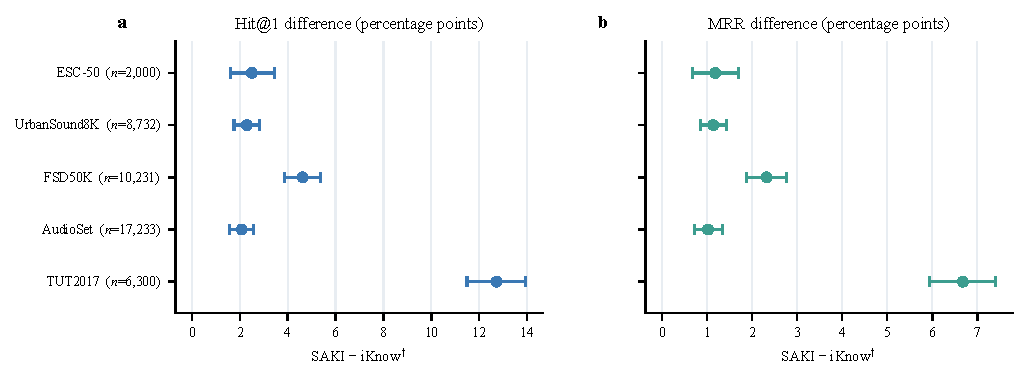
\includegraphics[width=\textwidth]{figures/further_analysis/fig_statistical_significance.pdf}
    \caption{\methodrevision{SAKI相对于iKnow\textsuperscript{\dag}的成对性能差值及95\%置信区间。圆点为观测到的指标差值，误差线为10,000次成对Bootstrap重采样得到的95\%置信区间；虚线表示零差值。}}
    \label{fig:statistical-significance}
\end{figure*}
\end{CJK*}

\subsection{Further analysis}\label{sec:further-analysis}
\begin{CJK*}{UTF8}{gbsn}

\methodrevision{本节进一步从统计差异、参数选择、计算成本及逐样本预测变化四个方面分析实验结果。统计分析报告性能差值的不确定性与Hit@1配对检验；参数分析说明开发集上的配置选择；成本分析量化在线推理和缓存开销；逐样本分析展示错误纠正与预测退化。}

\end{CJK*}

\subsubsection{Statistical significance}\label{sec:statistics}
\begin{CJK*}{UTF8}{gbsn}

\methodrevision{本文在同一批测试音频上比较SAKI与iKnow\textsuperscript{\dag}的Hit@1和MRR。为估计指标差值的抽样不确定性，以音频为单位进行10,000次成对Bootstrap重采样：每次有放回地抽取样本，并对两种方法使用相同的样本索引。重算每次的指标差值后，以其第2.5和97.5百分位数构建95\%置信区间。该区间反映测试样本抽样变化，不代表重新训练模型的波动。}

\methodrevision{如图~\ref{fig:statistical-significance}所示，本文方法在五个测试集上的Hit@1和MRR差值均为正，且对应的95\%置信区间均未跨越零。具体而言，Hit@1的提升范围为2.08--12.73个百分点，其中TUT2017的提升最大，较iKnow\textsuperscript{\dag}提高12.73个百分点，其95\%置信区间为[11.49, 13.95]。其余数据集的Hit@1提升分别为ESC-50上的2.50个百分点、UrbanSound8K上的2.29个百分点、FSD50K上的4.62个百分点以及AudioSet上的2.08个百分点。MRR呈现一致趋势，其提升范围为1.02--6.68个百分点。}



\methodrevision{对于Hit@1，本文另采用双侧精确McNemar检验，比较同一音频上“iKnow\textsuperscript{\dag}错误、SAKI正确”与“iKnow\textsuperscript{\dag}正确、SAKI错误”两类不一致配对的数量。这两类样本亦展示于图~\ref{fig:prediction-transitions}。对五个测试集分别检验后，采用Holm方法校正五个$p$值，以控制多重比较导致的第一类错误风险；校正后的$p$值均小于0.05。McNemar检验仅针对Hit@1正误，MRR差值的抽样不确定性则由上述Bootstrap区间表征。}

\end{CJK*}

\subsubsection{Parameter sensitivity}\label{sec:parameters}
\begin{CJK*}{UTF8}{gbsn}

本文进一步在DCASE17-T4开发集上分析了融合权重$\alpha$和样本级关系保留数量$N_r$对分类性能的影响。参数搜索范围设置为
\begin{equation}
\alpha\in\{0.3,0.5,0.7\},\qquad
N_r\in\{1,3,5,10\}.
\end{equation}
其余模型结构、知识检索设置和评价流程均保持不变。参数选择首先最大化Hit@1；当Hit@1相同时，进一步选择MRR较高的配置；若两项指标仍然相同，则优先选择关系数量较少的配置。

\begin{figure}[H]
    \centering
    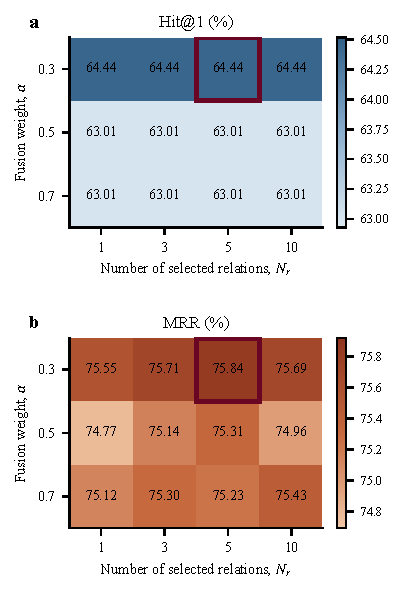
\includegraphics[width=0.96\columnwidth]{figures/further_analysis/fig_parameter_sensitivity.pdf}
    \caption{DCASE17-T4开发集上的参数敏感性分析。（a）不同融合权重$\alpha$和关系数量$N_r$下的Hit@1；（b）相同配置下的MRR。方框表示最终选择的参数组合$\alpha=0.3$和$N_r=5$。}
    \label{fig:parameter-sensitivity}
\end{figure}

\methodrevision{图~\ref{fig:parameter-sensitivity}(a)显示，在每个固定的$\alpha$值下，$N_r=1,3,5,10$的Hit@1相同。当$\alpha=0.3$时，Hit@1为64.44\%；当$\alpha=0.5$或$0.7$时，均为63.01\%。因此，在本开发集和所考察的范围内，改变$N_r$没有改变Hit@1正确样本数，而$\alpha=0.3$取得了较高的Hit@1。}

\methodrevision{图~\ref{fig:parameter-sensitivity}(b)进一步表明，相同Hit@1下的MRR仍随$N_r$变化。当$\alpha=0.3$时，$N_r=1,3,5,10$对应的MRR分别为75.55\%、75.71\%、75.84\%和75.69\%。按照先比较Hit@1、并列时再比较MRR的开发集选择规则，最终选定$\alpha=0.3$和$N_r=5$，并将其固定用于五个测试集。}

\end{CJK*}

\subsubsection{Computational cost analysis}\label{sec:computational-cost}
\begin{CJK*}{UTF8}{gbsn}

为量化知识增强的在线计算成本，本文在相同硬件和测试样本上比较CLAP、iKnow\textsuperscript{\dag}与SAKI。每个测试集从最终测试记录中固定选取200条样本，预热20条后重复计时5次。在线时间包括音频预处理、CLAP音频编码以及各方法的评分与排序；RotatE尾实体检索、AAKV文本生成和文本特征构建均属于离线预处理，不计入在线时间。表~\ref{tab:computational-cost}给出batch size为1时五个测试集的等权平均结果。

\end{CJK*}

\begin{table}[H]
\centering
\begin{CJK*}{UTF8}{gbsn}
\caption{Batch size为1时的在线推理效率与离线缓存规模。各数值为五个测试集的等权平均；相对开销以CLAP的平均延迟为基准。}
\label{tab:computational-cost}
\small
\setlength{\tabcolsep}{4pt}
\begin{tabular}{lccc}
\toprule
指标 & CLAP & iKnow\textsuperscript{\dag} & SAKI \\
\midrule
延迟（ms/样本） & 24.37 & 25.16 & 86.52 \\
相对开销 & 1.00$\times$ & 1.03$\times$ & 3.55$\times$ \\
吞吐量（样本/秒） & 41.03 & 39.74 & 11.56 \\
峰值GPU显存（MiB） & 693.60 & 700.30 & 743.22 \\
离线缓存（MiB） & 0.63 & 6.74 & 50.52 \\
\bottomrule
\end{tabular}
\end{CJK*}
\end{table}

\begin{CJK*}{UTF8}{gbsn}

如表~\ref{tab:computational-cost}所示，SAKI的平均在线延迟为86.52 ms/样本，是CLAP的3.55倍；iKnow\textsuperscript{\dag}的延迟为25.16 ms/样本，与CLAP的24.37 ms/样本接近。SAKI的平均峰值GPU显存和离线缓存规模也更高，表明前述分类性能增益伴随额外的在线计算与存储成本。

\end{CJK*}

\subsubsection{Prediction transitions and case study}\label{sec:cases}
\begin{CJK*}{UTF8}{gbsn}

\methodrevision{图~\ref{fig:prediction-transitions}进一步展示逐样本Hit@1预测转移。两组柱形分别表示“iKnow\textsuperscript{\dag}错误、SAKI正确”和“iKnow\textsuperscript{\dag}正确、SAKI错误”的样本数，也正是前述McNemar检验所比较的两类不一致配对。五个测试集上的前者均多于后者，ESC-50、UrbanSound8K、FSD50K、AudioSet和TUT2017分别净增加50、200、473、358和802个Hit@1正确样本。}

\begin{figure}[H]
    \centering
    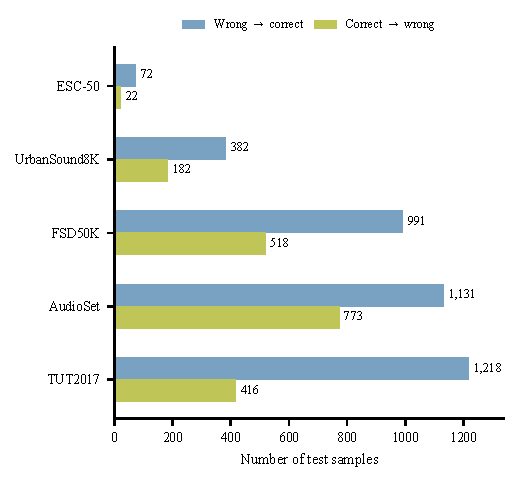
\includegraphics[width=\columnwidth]{figures/further_analysis/fig_prediction_transitions.pdf}
    \caption{\methodrevision{iKnow\textsuperscript{\dag}与SAKI之间的逐样本Hit@1预测转移。蓝色柱表示由错误转为正确的样本数，黄绿色柱表示由正确转为错误的样本数；两组数量构成McNemar检验的不一致配对。}}
    \label{fig:prediction-transitions}
\end{figure}

表~\methodrevision{\ref{tab:case-study}}进一步列出了ESC-50上的三类代表性样本，包括错误纠正、真实类别排名改善和正确预测退化。对于错误纠正样本，iKnow\textsuperscript{\dag}将真实类别\textit{wind}排在第5位并预测为\textit{train}，本文方法将\textit{wind}提升至第1位。在排名改善样本中，真实类别\textit{sea waves}由第3位提升至第2位，但最终预测仍为\textit{frog}。对于预测退化样本，iKnow\textsuperscript{\dag}能够正确识别\textit{washing machine}，而本文方法将\textit{engine}排在首位，使真实类别下降至第4位。

\begin{table}[!htbp]

\centering

\caption{ESC-50上的代表性逐样本预测变化。括号内为真实类别排名；每个案例展示一条代表性AAKV证据。}

\label{tab:case-study}

\footnotesize

\setlength{\tabcolsep}{2.4pt}

\begin{tabular}{p{1.05cm}p{1.15cm}p{1.45cm}p{1.45cm}}

\toprule

案例 & 真实类别 & iKnow\textsuperscript{\dag} & 本文方法 \\

\midrule

错误$\rightarrow$正确
& wind & train (5) & wind (1) \\

\multicolumn{4}{p{7.3cm}}
{\textit{AAKV evidence: The sound of wind is instance of ocean.}} \\

\addlinespace[2pt]

排名改善
& sea waves & crickets (3) & frog (2) \\

\multicolumn{4}{p{7.3cm}}
{\textit{AAKV evidence: The sound of frog is part of a wetland scene.}} \\

\addlinespace[2pt]

正确$\rightarrow$错误
& washing machine & washing machine (1) & engine (4) \\

\multicolumn{4}{p{7.3cm}}
{\textit{AAKV evidence: The sound of engine is instance of motorcycle.}} \\

\bottomrule

\end{tabular}

\end{table}

上述案例显示，本文方法通过改变候选类别的相对排序产生性能变化：真实类别既可能由较低排名提升至首位，也可能只获得有限的排名改善，或由首位下降至较低位置。结合图~\methodrevision{\ref{fig:prediction-transitions}}，五个测试集上的正向转移数量均高于负向转移数量。因此，本文方法的总体增益表现为逐样本排序变化所形成的净正向改善，同时仍存在预测退化的个别情况。
\end{CJK*}
\FloatBarrier

\section{Discussion}\label{sec:discussion}
\begin{CJK*}{UTF8}{gbsn}

\nextrevision{本文结果表明，图谱知识能否改善零样本音频分类，不仅取决于是否提供了类别名称之外的信息，还与关系选择、知识表达及分数融合方式有关。SAKI分别从这三个环节组织知识增强过程，完整配置取得最高的五数据集等权平均Hit@1和MRR，支持三个模块在总体表现上的互补作用。这些结果说明，在补充图谱知识的同时，还需要考虑如何针对当前音频选择关系、表达关系语义，以及协调知识证据与原始CLAP预测。}

\nextrevision{AAKV的作用需要分别从语言化对照和组合消融理解。在相同的关系选择与融合配置下，AAKV的Hit@1在五个测试集上均高于直接拼接和原始三元组表示，支持其在该配置下作为知识文本表示方式的有效性。AAKV保留三元组中的实体和关系方向，并将其组织为面向声音的文本，为CLAP利用关系语义提供了更明确的表达。另一方面，组合消融显示，AAKV单独启用时平均增益有限，且部分数据集的性能下降；与其他模块共同使用后，完整配置取得最高的五数据集等权平均Hit@1和MRR。这些结果表明，AAKV在不同模块配置下的收益存在差异，其单独使用的效果不足以概括其在完整方法中的贡献。}

\nextrevision{关系选择对照进一步支持了样本级关系选择的设计。在相同知识表示和融合配置下，该策略优于所比较的固定、高频和随机关系策略；所选关系组合的多样性也表明，选择结果随输入音频发生变化。前者支持其分类有效性，后者体现其样本依赖性。iKnow-audio采用经过筛选的关系集合检索尾实体，以扩展类别提示\,\cite{olvera-etal-2025-iknow}；SAKI则进一步依据当前音频下关系专家的预测共识与分类间隔，执行样本级关系选择，使参与知识增强的关系能够随输入调整。}

\nextrevision{不同评价指标的变化揭示了知识增强的收益边界。FSD50K上，在AAKV与样本级关系选择的组合中加入分层融合后，Hit@1基本持平，MRR略有提高；TUT2017上，完整方法相较于iKnow\textsuperscript{\dag}提高了Hit@1和MRR，但Hit@5略有下降。本文主要以Hit@1和MRR评价首位分类表现与真实类别的排序质量，并通过Hit@3和Hit@5补充考察前若干候选类别对真实标签的覆盖情况。因此，上述结果支持完整方法在本文主要评价指标上的总体优势，同时表明这种优势并未同步体现在所有评价指标上。逐样本分析同样观察到错误纠正、排名改善和预测退化，且五个测试集上的正向预测转移数量均超过负向转移数量，说明总体性能提升体现为逐样本排序变化带来的净改善。}

\nextrevision{SAKI仍受到知识质量、基础模型和计算成本的约束。AAKV能够约束三元组的文本表达，但不能校正三元组本身的错误；关系选择与知识评分也依赖CLAP对音频和文本的匹配能力。此外，尽管尾实体检索、AAKV文本生成和文本编码均在离线阶段完成并缓存，在线关系专家评估仍带来额外开销。当前测量中，SAKI的平均在线延迟为86.52 ms/样本，是CLAP的3.55倍，说明性能提升伴随着计算和存储成本的增加。当前结论基于固定的CLAP模型、RotatE评分函数及候选关系池；后续可考察证据可信度评估能否减少预测退化、轻量级关系预筛选能否降低在线开销，并在其他音频--语言模型与知识图谱上验证方法的适用范围。}

\end{CJK*}

\section{Conclusion}\label{sec:conclusion}
\begin{CJK*}{UTF8}{gbsn}

\methodrevision{本文围绕结构化知识如何适配当前音频并有效参与零样本分类的问题，提出了样本自适应知识整合框架SAKI。该框架通过样本级关系选择确定参与知识增强的关系，利用AAKV将图谱三元组转换为受约束的声音描述，并采用分层证据融合协调知识证据与原始CLAP预测对最终类别排序的贡献。在五个测试集上，SAKI相较于本文复现的iKnow-audio将Hit@1提高了2.08--12.73个百分点，MRR提高了1.02--6.68个百分点。完整因子消融、关系选择对照和知识语言化实验表明，三个模块在五数据集等权平均指标上具有互补作用，但单项数据集的增益并非完全一致。}

本文结果说明，结构化知识在零样本音频分类中的作用不仅取决于图谱是否包含相关实体，还取决于所选知识关系是否能够为当前样本提供有效的判别信息、关系语义能否被音频–文本模型有效表示，以及知识分数能否以适当方式参与最终决策。SAKI为将音频中心知识图谱转化为样本相关的分类证据提供了一种可行方案。当前结论适用于本文采用的CLAP模型、RotatE知识图谱表示及候选关系池；未来可通过证据可信度评估、关系预筛选以及跨模型和跨知识图谱验证，进一步提高知识增强分类的可靠性与适用范围。

\end{CJK*}


\section*{Acknowledgements}
This work was supported in part by the Wenzhou Basic Scientific Research Projects under Grant 2025G0082.

\section*{Declaration of competing interest}
The authors declare that they have no known competing financial interests or personal relationships that could have appeared to influence the work reported in this paper.

\section*{Data availability}
The datasets used in this study are publicly available, including ESC-50, UrbanSound8K, DCASE17-T4, FSD50K, AudioSet, and TUT2017. The processed data and implementation details will be made available by the corresponding authors upon reasonable request.

\bibliographystyle{elsarticle-num}
\bibliography{references}

% KBS/Elsevier appendices follow the reference list.
\appendix
% !TeX root = ../main.tex
\section{Additional ablation results}\label{app:ablation}
\setcounter{table}{0}
\renewcommand{\thetable}{A.\arabic{table}}
\begin{CJK*}{UTF8}{gbsn}

表~\ref{tab:ablation-topk}补充报告了正文完整因子消融实验的Hit@3和Hit@5结果。实验分支及其余配置均与表~\ref{tab:factorial-ablation}保持一致。

\begin{table*}[t]
\centering
\caption{完整因子消融实验的Hit@3和Hit@5结果（\%）。数值越高越好；实验分支与其余配置均与表~\ref{tab:factorial-ablation}一致。}
\label{tab:ablation-topk}
\setlength{\tabcolsep}{2.5pt}
\resizebox{\textwidth}{!}{%
\begin{tabular}{l*{12}{c}}
\toprule
\multirow{2}{*}{方法}
& \multicolumn{2}{c}{ESC-50}
& \multicolumn{2}{c}{UrbanSound8K}
& \multicolumn{2}{c}{FSD50K}
& \multicolumn{2}{c}{AudioSet}
& \multicolumn{2}{c}{TUT2017}
& \multicolumn{2}{c}{\methodrevision{五数据集等权平均}} \\
\cmidrule(lr){2-3}\cmidrule(lr){4-5}\cmidrule(lr){6-7}\cmidrule(lr){8-9}\cmidrule(lr){10-11}\cmidrule(lr){12-13}
& Hit@3 & Hit@5 & Hit@3 & Hit@5 & Hit@3 & Hit@5 & Hit@3 & Hit@5 & Hit@3 & Hit@5 & Hit@3 & Hit@5 \\
\midrule
iKnow\textsuperscript{\dag}
& 97.05 & 97.65 & 96.77 & 98.65 & 80.73 & 86.51 & 47.04 & 54.87 & 79.89 & 92.68 & 80.30 & 86.07 \\
+ AAKV
& 95.90 & 97.65 & 96.14 & 98.65 & 80.63 & 86.46 & 46.73 & 54.80 & 79.65 & 92.27 & 79.81 & 85.97 \\
+ Hierarchical Fusion
& 97.10 & 97.65 & 96.86 & 98.65 & 81.24 & 86.67 & 47.48 & 55.14 & 80.78 & 92.65 & 80.69 & 86.15 \\
+ Relation Selection
& 97.05 & 97.70 & 96.36 & 98.65 & 79.96 & 86.38 & 46.68 & 55.00 & 80.83 & 92.52 & 80.17 & 86.05 \\
+ AAKV + Fusion
& 97.00 & 97.65 & 96.56 & 98.65 & 81.21 & 86.58 & 47.10 & 54.93 & 81.30 & 92.00 & 80.64 & 85.96 \\
+ AAKV + Relation Selection
& 96.30 & 97.65 & 96.09 & 98.65 & \methodrevision{80.09} & \methodrevision{86.40} & \methodrevision{46.61} & 54.90 & 79.56 & 92.25 & \methodrevision{79.73} & 85.97 \\
+ Fusion + Relation Selection
& 97.05 & 97.65 & 96.60 & 98.65 & 79.68 & 86.38 & 46.34 & 54.94 & 80.70 & 92.63 & 80.07 & 86.05 \\
完整方法
& 96.80 & 97.65 & 96.90 & 98.65 & \methodrevision{80.52} & \methodrevision{86.48} & \methodrevision{46.90} & \methodrevision{54.80} & 80.54 & 91.79 & \methodrevision{80.33} & 85.88 \\
\bottomrule
\end{tabular}
}
\end{table*}

\begin{table*}[t]
\centering
\caption{Frequency Top-5在各数据集上选择的关系。该策略仅依据离线知识缓存中的类别--尾实体证据数量，不使用输入音频、音频标签或测试集真值。}
\label{tab:frequency-relations}
\setlength{\tabcolsep}{4pt}
\begin{tabular}{lp{0.82\textwidth}}
\toprule
数据集 & Frequency Top-5关系 \\
\midrule
ESC-50 & \texttt{can be heard in}; \texttt{has duration}; \texttt{localized in}; \texttt{part of scene}; \texttt{associated with environment} \\
UrbanSound8K & \texttt{affects}; \texttt{associated with environment}; \texttt{associated with event}; \texttt{can be heard in}; \texttt{co-occurs with} \\
FSD50K & \texttt{associated with environment}; \texttt{can be heard in}; \texttt{localized in}; \texttt{occurs in}; \texttt{part of scene} \\
AudioSet & \texttt{can be heard in}; \texttt{occurs in}; \texttt{localized in}; \texttt{described by}; \texttt{associated with environment} \\
TUT2017 & \texttt{affects}; \texttt{associated with environment}; \texttt{can be heard in}; \texttt{co-occurs with}; \texttt{emotionally associated with} \\
\bottomrule
\end{tabular}
\end{table*}

\end{CJK*}

\onecolumn
\raggedbottom
\section{Reproduction Protocol and Dataset Reconciliation}\label{app:reproduction}
\enlargethispage{5\baselineskip}
\setcounter{table}{0}
\renewcommand{\thetable}{B.\arabic{table}}

\subsection{Dataset protocol reconciliation}

\begin{table}[H]
\centering
\caption{Dataset protocols used in iKnow-audio and in our experiments.}
\label{tab:dataset-reconciliation}
\fontsize{7.5}{8.2}\selectfont
\setlength{\tabcolsep}{4pt}
\begin{tabular}{lrrlp{0.55\textwidth}}
\toprule
Dataset & iKnow-audio & This work & Role & Protocol note \\
\midrule
ESC-50 & 2,000 & 2,000 & Test & The full dataset is used. All 2,000 files in our evaluation manifest pass the audio-readability audit. \\
UrbanSound8K & 8,732 & 8,732 & Test & The full dataset is used. All 8,732 files in our evaluation manifest pass the audio-readability audit. \\
FSD50K & 20,462 & 10,231 & Test & We use the official FSD50K evaluation split containing 10,231 clips. The iKnow-audio paper reports 20,462 test items; therefore absolute results across the two protocols are not treated as directly comparable. \\
AudioSet & 20,371 & 17,233 & Test & Our fixed evaluation manifest contains 17,233 available and readable audio files. The exact manifest will be released for reproducibility. \\
TUT2017 & 6,300 & 6,300 & Test & Final experiments use the complete development (4,680) and evaluation (1,620) partitions. Earlier 4,680-only results were replaced by the full 6,300-clip rerun. \\
DCASE17-T4 & 488 & 419 & Development & Our fixed development manifest contains 419 readable clips and is used only for selecting $\alpha$ and $N_r$. It is excluded from the five final test datasets. \\
\bottomrule
\end{tabular}
\end{table}

\subsection{iKnow\textsuperscript{\dag} controlled-reproduction protocol}

\begin{table}[H]
\centering
\caption{Reconciliation between the original iKnow-audio protocol and the controlled reproduction used in this work.}
\label{tab:iknow-protocol}
\fontsize{7.5}{8.2}\selectfont
\setlength{\tabcolsep}{4pt}
\begin{tabular}{p{0.16\textwidth}p{0.27\textwidth}p{0.23\textwidth}p{0.27\textwidth}}
\toprule
Component & Original iKnow-audio & iKnow\textsuperscript{\dag} in this work & Treatment \\
\midrule
Relation set & Uses a manually curated informative relation subset $R_q \subset R$ & Uses a reconstructed, dataset-specific fixed relation configuration & The complete original $R_q$ is not publicly specified; the reproduced configuration is explicitly denoted by \textsuperscript{\dag} \\
Knowledge graph & Audio-centric Knowledge Graph (AKG) & AKG resource used in our reproduction & Kept fixed across internal comparisons \\
KGE model & KGE-based tail prediction & RotatE & Kept fixed across internal comparisons \\
Candidate classes & CLAP top-ranked candidate classes & Top-$K$, $K=5$ & Unified across iKnow\textsuperscript{\dag} and ablation branches \\
Tail retrieval & Top-ranked tail entities & Top-$M$, $M=3$ & Unified across iKnow\textsuperscript{\dag} and ablation branches \\
Knowledge text & Class label combined with predicted knowledge entity & Direct class--tail concatenation & Used as the baseline knowledge-text representation \\
Score aggregation & LogSumExp over base and knowledge-enhanced scores & Normalized scaled LogSumExp, $\methodrevision{\lambda}=100$ & Controlled modification introduced in our reproduction \\
Evidence Top-P & Public configuration does not fully determine the final reproduced filtering setting & Disabled in the final protocol & Kept identical across final ablation branches \\
Test-label use & Not used during zero-shot inference & Not used during inference or relation selection & Labels are used only for evaluation \\
Evaluation samples & Original paper protocol & Fixed manifests in Table~\ref{tab:dataset-reconciliation} & All methods in this work use identical manifests and evaluation code \\
\bottomrule
\end{tabular}
\end{table}

\section{Sample-Adaptive Relation Selection Behavior}\label{app:selector-behavior}
\setcounter{table}{0}
\renewcommand{\thetable}{C.\arabic{table}}

\begin{table}[H]
\centering
\caption{Sample-level relation selection behavior on the five test datasets. Unique Top-5 sets and dominant-set share treat relation combinations as unordered. Mean Jaccard is computed against the complete dataset-specific FrozenRq set.}
\label{tab:selector-behavior}
\small
\setlength{\tabcolsep}{10pt}
\begin{tabular}{lrrrr}
\toprule
Dataset & \#Samples & \#Unique Top-5 sets & Dominant-set share (\%) & Mean Jaccard vs FrozenRq \\
\midrule
ESC-50 & 2,000 & 1,708 & 1.40 & 0.0405 \\
UrbanSound8K & 8,732 & 5,461 & 1.53 & 0.0739 \\
FSD50K & 10,231 & 9,066 & 1.51 & 0.0549 \\
AudioSet & 17,233 & 15,671 & 1.50 & 0.0577 \\
TUT2017 & 6,300 & 4,336 & 1.06 & 0.0636 \\
\bottomrule
\end{tabular}
\end{table}

\section{\methodrevision{AAKV Generation and Validation Protocol}}\label{app:aakv-protocol}

\methodrevision{For each retrieved triple, the generator receives a system instruction and a user message containing the three fields \texttt{[head]}, \texttt{[relation]}, and \texttt{[tail]}. The placeholder \texttt{\{head\}} in the instruction is replaced with the supplied head text. The full system instruction used in the implementation is reproduced below.}

\begin{quote}
\methodrevision{You are a faithful knowledge-graph verbalizer for an audio-text matching model. Convert exactly one knowledge-graph triple into one short, natural English sentence about sound.}

\methodrevision{Rules:}
\begin{enumerate}
\item \methodrevision{Begin the sentence with exactly: ``The sound of \texttt{\{head\}}''. Replace \texttt{\{head\}} with the supplied head text exactly.}
\item \methodrevision{Use only information explicitly contained in the triple.}
\item \methodrevision{Preserve the head entity, relation meaning, relation direction, and tail entity.}
\item \methodrevision{Preserve the original wording of the head and tail. Do not pluralize, abbreviate, replace, or omit either entity.}
\item \methodrevision{Do not add acoustic properties, causes, locations, purposes, examples, explanations, or external knowledge.}
\item \methodrevision{Do not correct or reinterpret the factual content, even if it seems unusual.}
\item \methodrevision{Add only grammatical function words such as articles, prepositions, and forms of ``be''.}
\item \methodrevision{Silently verify that the sentence expresses exactly the supplied triple.}
\item \methodrevision{Output only one final sentence, without reasoning, labels, headers, or quotation marks.}
\end{enumerate}
\end{quote}

\methodrevision{The user message has the exact field layout \texttt{[head] head}, \texttt{[relation] relation}, and \texttt{[tail] tail}, with each field on a separate line. Qwen2.5-7B-Instruct is decoded greedily (\texttt{do\_sample=False}, \texttt{max\_new\_tokens=48}). The rule-based check tests the required prefix, lexical coverage of the head and tail, relation-keyword coverage, a maximum of 30 words, a single line and sentence, and the absence of predefined extra-format or acoustic-property terms. These checks assess observable text constraints; they do not constitute a semantic proof of triple fidelity.}

\methodrevision{If the first output fails, the model receives its preceding output, the failed-check reasons, and the following repair instruction: ``Your preceding sentence failed an automatic fidelity check. Rewrite it as exactly one short English sentence beginning with the exact words `The sound of \texttt{\{head\}}'. Copy the supplied head and tail text exactly and explicitly express the supplied relation in its original direction. Do not add, correct, explain, or infer anything. Output only the sentence.'' If the repaired output still fails, the implementation uses the deterministic fallback ``The sound of \texttt{\{head\}} has the relation \texttt{\{relation\}} with \texttt{\{tail\}}.''}


\end{document}
